\pagestyle{myFancy}
\chapter{Computer Simulation of Pure Gauge Theories}
\section{Introduction}
Monte Carlo simulations are a powerful tool that can be used to evaluate observables in lattice field theory.
Given an observable $O$ (such as a plaquette, a Wilson or Polyakov loop, etc.), its vacuum expectation value is formally given by the functional integral
\begin{equation}
    \expval{O} = \frac1Z\int\DD[U]e^{-S[U]}O[U] \qquad \text{with} \qquad Z = \int\DD[U]e^{-S[U]}O[U] \label{2:Observable}
\end{equation}
where $\DD[U]$ is to be intended as a Haar measure.\\
This expression, however, cannot be evalued analytically except for very small lattices, therefore \eqref{2:Observable} is approximated by an average of the observable evaluated on $N$ sample gauge field configurations $\prc{U_n}$\footnote{Here the subscript $n$ distinguishes the different configurations.}, distributed according a probability density $\varpropto e^{-S[U_n]}$.\\
The expectation value is then obtained by computing the following sum for a sufficient number of configurations generated by the proper Monte Carlo algorithm(s):
\begin{equation}
    \expval{O} \simeq \frac1N\sum_{\prc{U_n}}O[U_n] \label{2:ExpValObs}
\end{equation}
Because of the probability density $\varpropto e^{-S[U_n]}$, only configurations $\prc{U_n}$ that minimize the action are \emph{good configurations}, as all other configurations are exponentially suppressed.
For this reason, generating totally random gauge fields on the lattice links is not an efficient way to evaluate \eqref{2:ExpValObs}, as most of the $\prc{U_n}$ will have a very small Boltzmann factor (the $e^{-S[U_n]}$) and expression \eqref{2:ExpValObs} will give incorrect results unless a huge number (orders of magnitude higher than what is reasonably possible) of different configurations is tried.\\
In order to avoid the evaluation of a great number of configurations that would contribute little-to-nothing to the observables' values, a sequence of configurations $\prc{U_n}$ is generated through a Markov chain process, built such that its stationary distribution minimizes the action $S[U]$. This process is usually called \emph{thermalization}.\\
Every process of this type must begin from a starting configuration, usually chosen by the user.
The two mostly used starting configurations are: a \emph{cold start}, if the simulation begins with the fields in an ordered way (for example, all the gauge links set to the identity), or a \emph{hot start}, if the simulation begins with random gauge fields in every link.
Of course, the Markov chain must have the same stationary distribution if the hot or cold start is chosen.\\
In this chapter the main Monte Carlo algorithms used to thermalize the starting configuration are presented, then the methods used for evaluating some observables of interest, such as plaquettes and Polyakov loops, are explained.

\section{Markov Processes}
As anticipated before, a Markov chain is needed to evolve an arbitrary starting configuration $U_0$ up to a region of the configuration space with a relatively large Boltzmann factor $e^{-S}$, therefore with high probability.
In Figure \eqref{2F:MarkovProcess} a scheme of a Markov chain is shown.
\begin{figure}[!htbp]
    \centering
    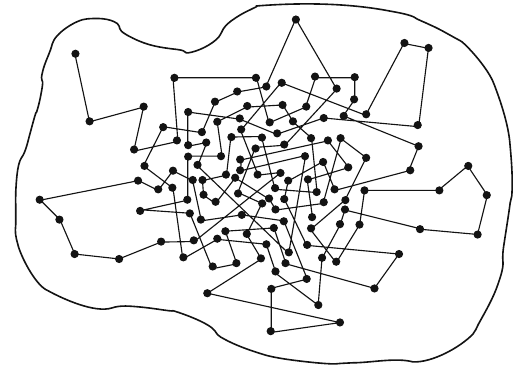
\includegraphics[width=0.5\textwidth]{MarkovProcess.png}
    \caption{Schematic representation of a motion throug the space of configurations through a Markov process.}
    \label{2F:MarkovProcess}
\end{figure}\\
A Markov process is charaterized by a probability of transitioning from a configuration $\alpha$ to another configuration $\beta$ depending only on $\alpha$ and $\beta$ and not on the history of the process, namely the previous transitions that already occourred.
In formulae, this is expressed as
\begin{equation}
    P(U_n=\beta|U_{n-1}=\alpha) = T(\beta|\alpha) \label{2:TransMatrix}
\end{equation}
That is to say that the transition matrix $T$ does not depend on the index $n$, representing the computer time.\\
Being a transition probability, the matrix $T$ must obey the following equations
\begin{align}
    0 \leq T(\beta|\alpha) \leq& 1 \qquad \forall \alpha,\beta \label{2:TPropProb} \\
    \sum_{\beta}T(\beta|\alpha) =& 1 \qquad \forall \alpha \label{2:TPropNorm}
\end{align}
where \eqref{2:TPropProb} is a consequence of $T(\beta|\alpha)$ representing a probability, and \eqref{2:TPropNorm} means that the probability of transitioning to any configuration must be $1$ (of course, the case when $\alpha=\beta$ is included as well).\\
In order for the stochastic process not to have any sink or source of probability, the following balance equation must be satisfied:
\begin{equation}
    \sum_\alpha T(\beta|\alpha)P(\alpha) = \sum_\alpha T(\alpha|\beta)P(\beta) \label{2:BalanceEq}
\end{equation}
This equation states that the probability of transitioning to the configuration $\beta$, written in the \lhs as the sum of the transition probability from the configuration $\alpha$ weighted by the probability $P(\alpha)$ that the system is actually in that configuration, must be equal to the probability of transitioning out of the configuration $\beta$, given by the probability of finding the system in the configuration $\beta$ times the transition probability $T(\alpha|\beta)$ over all the final configurations, in the right-hand side.
Thanks to \eqref{2:TPropNorm}, the \rhs is easily proven to be equal to $P(\beta)$.\\
A sufficient (but not necessary) condition to obey the balance equation \eqref{2:BalanceEq} is obtained by requiring that it holds true term-by-term, thus obtaining the detailed balance condition:
\begin{equation}
    T(\beta|\alpha)P(\alpha) = T(\alpha|\beta)P(\beta) \label{2:DetailedBalance}
\end{equation}
Although it is not a necessary condition, most algorithms, including the ones discussed in the following section, satisfy it.

\section{Monte Carlo Algorithms}
Monte Carlo algorithms are a class of algorithms that, singularly or combined together, allow to advance the Markov chain, while satisfying the balance condition \eqref{2:BalanceEq}.\\
Each algorithm, if applied once, allows the transition from a configuration $U_{n-1}$ to a configuration $U_n$ (eventually the same as $U_{n-1}$). The repeated application of the algorithm allows to advance through the Markov chain.

\subsection{Metropolis Algorithm}
The first algorithm presented is the Metropolis algorithm. It is not very much efficient and it is not often used in simulations unless for didactical purposes, however it contains the fundamental steps that are present in some of the more advanced algorithms and it is quite easy to understand.
For this reasons it is usually viewed as the \emph{``ancestor''} of all Monte Carlo algorithms and it is present in every textbook on the subject.\\
This algorithm consists in two steps that implement in one of the most simple ways the detailed balance condition \eqref{2:DetailedBalance}:
\begin{enumerate}[label=\arabic*)]
    \item A candidate configuration $\beta$ is chosen, according to some \emph{a priori} selection probability $T_0(\beta|\alpha)$, where $\alpha=U_{n-1}$.
    \item The candidate configuration $\beta$ is accepted as the new configuration $U_n$ with the acceptance probability
          \begin{equation}
              T_A(\beta|\alpha) = \min\pr{1,\frac{T_0(\alpha|\beta)\exp(-S[\beta])}{T_0(\beta|\alpha)\exp(-S[\alpha])}} \label{2:MetropolisAccProb}
          \end{equation}
          If it is not accepted, the unchanged configuration is considered again ($U_n=\alpha$) and the measurements are eventually made again.
\end{enumerate}
These two steps are repeated a sufficient amount of times up unitl the needed measurements are taken.\\
Note that $P(\alpha) = \frac{e^{-S[\alpha]}}{Z} \varpropto e^{-S[\alpha]}$ has been used.\\
The total transition probability $T$ is obtained through the product $T=T_0T_A$, as the two steps are independant from each other, and it is straightforward to see that it satisfies the detailed balance condition \eqref{2:DetailedBalance}:
\begin{align*}
    T(\beta|\alpha)P(\alpha) =& \frac1Z T_0(\beta|\alpha)T_A(\beta|\alpha)\exp(-S[\alpha]) = \\
    =& \frac1Z T_0(\beta|\alpha)\min\pr{1,\frac{T_0(\alpha|\beta)\exp(-S[\beta])}{T_0(\beta|\alpha)\exp(-S[\alpha])}}\exp(-S[\alpha]) = \\
    =& \frac1Z \min\pr{T_0(\beta|\alpha)\exp(-S[\alpha]), T_0(\alpha|\beta)\exp(-S[\beta])} = \\
    =& \frac1Z T(\alpha|\beta)\exp(-S[\beta]) = \\
    =& T(\alpha|\beta)P(\beta)
\end{align*}
\qed
In many cases a symmetric selection probability is used $T_0(\alpha|\beta)=T_0(\beta|\alpha)$, thus \eqref{2:MetropolisAccProb} simpliefies to:
\begin{equation}
    T_A(\beta|\alpha) = \min\pr{1, e^{-\Delta S}} \quad \text{with} \quad \Delta S = S[\beta]-S[\alpha] \label{2:MetropolisAccProbSymm}
\end{equation}
That means that if the new configuration lowers the action, the change is accepted with probability $1$ (as $e^{-\Delta S}>1$), otherwise it is accepted with a certain probability that decays exponentially as the difference in the action of the two configurations becomes greater.
This ensures that the algorithm \emph{moves across} the configuration space towards the minimums of the action, while allowing quantum fluctuations in order to not \emph{``get stuck''} on a local minimum.\\
If the change in the action is local (it involves a single link variable), $\Delta S$ can be computed using only the field values in the local neighbour. This will be the case for $\SUN$ gauge theories.

\subsubsection{Application to SU(N) Gauge Theories}
For a $\SUN$ gauge theory, the algorithm is implemented in the following way.
During each iteration, a single link is changed, then the acceptance probability is computed, a random number is extracted and, if it is less than the acceptance probability the change is accepted, otherwise it is rejceted.
The algorithm is then iterated a certain number of times and measures are taken.\\
The candidate link $U'_\mu(x)$ for step 1 is generated in the vicinity of the old value $U_\mu(x)$, in order not to have a too great $\Delta S$ that would lead to too low acceptance rates.
This can be done by exploiting the property that the product of any two elements of $\SUN$ is still an element of $\SUN$, therefore extracting a matrix $X\in\SUN$ near the identity allows to write the candidate link as:
\begin{equation}
    U'_\mu(x) = XU_\mu(x) \label{2:MetropolisCandidateLink}
\end{equation}
The matrix $X$ is chosen such that it has the same probability as $X^{-1}$, this way the selection probability $T_0$ is symmetric and the computation of the acceptance probability $T_A$ becomes easier.\\
For this reason, only the variation of the action $\Delta S$ must be computed, where of course the action is the Wilson action \eqref{1:WilsonAction}.
In particular, only the plaquettes containing the candidate link must be evaluated: the change in the action is local, so all the other plaquettes will have the same value both before and after the change of the link.
Hence $\Delta S = S[U'_\mu(x)]_{loc}-S[U_\mu(x)]_{loc}$.\\
In a SH lattice, each link is shared between $6$ plaquettes, in $4$ spacetime dimensions.
For each plaquette the change of its value is given by the change of the link, while the product of the other three gauge links, that is called \emph{staple} and will be indicated as $P_i$, remains unchanged.\\
\begin{figure}[!htbp]
    \centering
    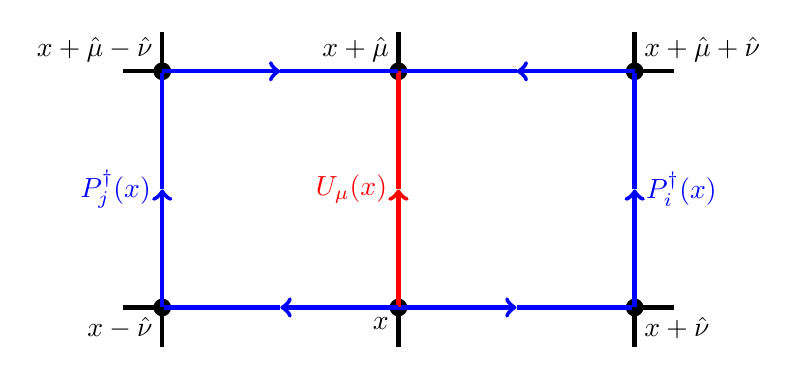
\begin{tikzpicture}
        \filldraw[black]  (0,0) circle (3pt) node[anchor=north east]{$x$};
        \filldraw[black]  (0,3) circle (3pt) node[anchor=south east]{$x+\hat\mu$};
        \filldraw[black]  (3,0) circle (3pt) node[anchor=north west]{$x+\hat\nu$};
        \filldraw[black]  (3,3) circle (3pt) node[anchor=south west]{$x+\hat\mu+\hat\nu$};
        \filldraw[black] (-3,0) circle (3pt) node[anchor=north east]{$x-\hat\nu$};
        \filldraw[black] (-3,3) circle (3pt) node[anchor=south east]{$x+\hat\mu-\hat\nu$};
        \draw[ultra thick] (0,-0.5) -- (0,0);
        \draw[color=blue,ultra thick,->] (0,0) -- (1.5,0);
        \draw[color=blue,ultra thick   ] (1.5,0) -- (3,0);
        \draw[ultra thick]  (3.5,0) -- (3,0);
        \draw[ultra thick] (3,-0.5) -- (3,0);
        \draw[color=blue,ultra thick,->] (3,0) -- (3,1.5) node[anchor=west]{$P^\dagger_i(x)$};
        \draw[color=blue,ultra thick   ] (3,1.5) -- (3,3);
        \draw[ultra thick]  (3.5,3) -- (3,3);
        \draw[ultra thick]  (3,3.5) -- (3,3);
        \draw[color=blue,ultra thick,->] (3,3) -- (1.5,3);
        \draw[color=blue,ultra thick   ] (1.5,3) -- (0,3);
        \draw[ultra thick]  (0,3.5) -- (0,3);
        \draw[color=red,ultra thick,->] (0,0) -- (0,1.5) node[anchor=east]{$U_\mu(x)$};
        \draw[color=red,ultra thick   ] (0,1.5) -- (0,3);
        
        \draw[color=blue,ultra thick,->] (0,0) -- (-1.5,0);
        \draw[color=blue,ultra thick   ] (-1.5,0) -- (-3,0);
        \draw[ultra thick]  (-3.5,0) -- (-3,0);
        \draw[ultra thick] (-3,-0.5) -- (-3,0);
        \draw[color=blue,ultra thick,->] (-3,0) -- (-3,1.5) node[anchor=east]{$P^\dagger_j(x)$};
        \draw[color=blue,ultra thick   ] (-3,1.5) -- (-3,3);
        \draw[ultra thick]  (-3.5,3) -- (-3,3);
        \draw[ultra thick]  (-3,3.5) -- (-3,3);
        \draw[color=blue,ultra thick,->] (-3,3) -- (-1.5,3);
        \draw[color=blue,ultra thick   ] (-1.5,3) -- (-0,3);
    \end{tikzpicture}
    \caption{Example of a link (\textcolor{red}{red}) with two of its staples (\textcolor{blue}{blue}).}
    \label{2F:Staple}
\end{figure}\\
Therefore, the local contribution to the action can be computed as:
\begin{equation*}
    S[U_\mu(x)]_{loc} = \frac\beta{2N} \sum_{i=1}^6 \Re\Tr\prs{\id-U_\mu(x)P_i} = \frac\beta{2N} \Re\Tr\prs{6\id-U_\mu(x)\sum_{i=1}^6P_i}
\end{equation*}
where the sum over all the staples is:
\begin{equation}
    A = \sum_{i=1}^6P_i = \sum_{\nu\neq\mu}\pr{U_\nu(x+\hat\mu)U^\dagger_\mu(x+\hat\nu)U^\dagger_\nu(x) + U^\dagger_\nu(x+\hat\mu)U^\dagger_\mu(x-\hat\nu)U_\nu(x-\hat\nu)} \label{2:SumOverStaples}
\end{equation}
The change of the action can now be computed as
\begin{equation}
    \Delta S = S[U'_\mu(x)]_{loc}-S[U_\mu(x)]_{loc} = \frac\beta{2N} \Re\Tr\prs{\pr{U_\mu(x)-U'_\mu(x)}A} \label{2:MetropolisActionVar}
\end{equation}
where $A$ is not affected by the change of $U_\mu(x)$.

\subsection{Heat Bath Algorithm}
The heat bath algorithm is an \emph{enhanced} version of the Metropolis algorithm, that combines the two steps into a single one and chooses the new candidate according to the probability distribution obtained by the computing the surrounding staples:
\begin{equation}
    \dd P(U) = \dd U \exp(\frac\beta{2N}\Re\Tr[U A]) \label{2:DistrProbHB}
\end{equation}
where $\dd U$ denotes the Haar integration measure of the gauge group and $A$ is computed according to \eqref{2:SumOverStaples}.
This probability distribution can be computationally quite demanding, but has the advantage that, unlike the Metropolis algorithm, the link variable always changes.\\
The implementation details depend on the gauge group, for this reason, the heat bath method for the gauge group $\SU(2)$ will be now explained\footnote{As matrixes of $\SUN$ can be ``built'' combining $\SU(2)$ matrixes, the general case is just a little more complicated, but it follows the same principles.}.\\
Since the sum of any two $\SU(2)$ elements is proportional to another $\SU(2)$ element, the sum of all staples $A$ \eqref{2:SumOverStaples} can be written in the form
\begin{equation}
    A = V\sqrt{\det(A)} \qquad\text{with}\qquad V\in\SU(2) \label{2:SumOverStaplesSU2}
\end{equation}
where it can be proven that $\det(A)\geq0$.
If $\det(A)=0$, a random link variable is generated, otherwise the matrix $V$ is well-defined.
Plugging into \eqref{2:DistrProbHB} and using the invariance of the Haar measure under trasformation of the origin of the group space ($\dd U = \dd (UV) = \dd X$), the distribution probability of the matrix $X=UV$ is
\begin{equation}
    \dd P(X) = \dd X \exp(\frac\beta{2N}\sqrt{\det(A)}\Re\Tr[X]) \label{2:DistrProbHBX}
\end{equation}
If a matrix $X$, distributed according to \eqref{2:DistrProbHBX}, is generated, then the new candidate link, distributed according to \eqref{2:DistrProbHB}, is obtained as $U'_\mu(x) = XV^\dagger = \frac1{\sqrt{\det(A)}}XA^\dagger$.\\
Any $U\in\SU(2)$ matrix can be written in the following representation, using $4$ real numbers:
\begin{equation}
    U=x_0\id+\i \bm{x} \cdot \bm{\sigma} \qquad\text{with}\qquad \det(U)=\abs{x}^2=\sum_{i=0}^3x_i^2=1 \label{2:SU2Repr}
\end{equation}
where $\bm\sigma=\pr{\sigma_1,\sigma_2,\sigma_3}$ is a vector built using the Pauli matrixes and $x=(x_0,\bm{x})$ can be seen as a normalized $4$-compnents vector.
Using this representation, the Haar measure in \eqref{2:DistrProbHBX} can be written as:
\begin{align*}
    \dd X =& \frac1{\pi^2} \dd^4x \delta\pr{x_0^2+\bm{x}-1} =\\
    =& \frac1{\pi^2} \dd^4x \frac{1}{2\sqrt{1-x_0^2}} \pr{\delta\pr{\abs{\bm{x}}-\sqrt{1-x_0^2}}+\delta\pr{\abs{\bm{x}}+\sqrt{1-x_0^2}}} \numthis\label{2:HaarMeasureHB}
\end{align*}
where a well known property of the Dirac delta function has been used.\\
The volume element can be rewritten in terms of the components of the vector $x$:
\begin{equation}
    \dd^4x = \dd x_0\dd\abs{\bm{x}}\abs{\bm{x}}^2\underbrace{\dd(\cos\theta)\dd\varphi}_{\dd^2\Omega} \label{2:VolumeElemParam}
\end{equation}
Plugging back into \eqref{2:HaarMeasureHB} and integrating out the $\abs{\bm{x}}$ thanks to the delta functions (actually, only the first one contributes, as $x_i^2\leq1$ $\forall i$), the Haar measure takes the form:
\begin{equation}
    \dd X = \frac1{\pi^2}\dd x_0\dd^2\Omega\frac{1-x_0^2}{2\sqrt{1-x_0^2}} = \frac1{2\pi^2} \dd x_0 \dd^2\Omega \sqrt{1-x_0^2} \label{2:HaarMeasureHBSimplified}
\end{equation}
Then, in terms of the variables, the probability distribution becomes:
\begin{equation}
    \dd P(X) = \frac1{2\pi^2} \dd x_0 \dd(\cos\theta) \dd\varphi \sqrt{1-x_0^2} \exp\pr{\frac\beta2 \sqrt{\det(A)}x_0} \label{2:DistrProbHBXSimplified}
\end{equation}
with $x_0\in[-1,1]$, $\cos\theta\in[-1,1]$, $\varphi\in[0,2\pi)$, where $\Tr(X)=2x_0$ has been used.\\
Thus, the problem of generating a matrix $X$ distributed according to \eqref{2:DistrProbHBX} has been reduced to the determination of three random variables $x_0$, $\theta$, $\varphi$, whose distributions factorize, so they can be determined independetly from each other.\\
The random variable $x_0$, being distributed according to $\sqrt{1-x_0^2} \exp\pr{\frac\beta2 \sqrt{\det(A)}x_0}$, is determined through the auxiliary variable $\lambda\in[0,1]$ such that $x_0 = 1-2\lambda^2$, therefore
\begin{equation}
    \dd x_0\sqrt{1-x_0^2} \exp\pr{\frac\beta2 \sqrt{\det(A)}x_0} \varpropto \dd\lambda\lambda^2\sqrt{1-\lambda^2} \exp\pr{-\beta \sqrt{\det(A)}\lambda^2} \label{2:LambdaDistrHB}
\end{equation}
The variable $\lambda$ is generated with the polynomially modified Gaussian distribution density
\begin{equation}
    p_1(\lambda) = \lambda^2 e^{-\beta \sqrt{\det(A)}\lambda^2}
\end{equation}
and accepted with an accept/reject step using the square root function
\begin{equation}
    p_2(\lambda) = \sqrt{1-\lambda^2}
\end{equation}
There are several algorithms that can perform this computation in an efficient way~\cite{1998art, luscher1994portable}.\\
After this, the length $\abs{x} = \sqrt{1-x_0^2}$ is computed, in order to determine the remaining variables.\\
The variables $\cos\theta$ and $\varphi$ are uniformely distributed, therefore a possible way of proceeding is by generating three random uniformely distributed numbers $r_1$, $r_2$ and $r_3$ in the interval $[-1,1)$ and accepting them only if $r_1^2+r_2^2+r_3^2\leq1$.
Then, the $3$-vector $(r_1,r_2,r_3)$ is normalized to length $\abs{x}$ computed before, obtaining $\bm{x} = (x_1,x_2,x_3)$.\\
After these steps, the vector $x=(x_0,\bm{x})$ can be used to generate the matrix $X$ according to \eqref{2:DistrProbHBX}, using representation \eqref{2:SU2Repr}, thus the new link variable can be obtained.\\
This algorithm rapidly leads the Markov process to a minimum of the action, however the risk of ``getting stuck'' on a local minimum is present.
For this reason, it is usually combined with other algorithms, like the overrelaxation algorithm.

\subsection{Overrelaxation Algorithm}
The overrelaxation algorithm tries to change the link variables as much as possible, exploiting the property that new configurations are always accepted if they do not change the action, as can be seen in \eqref{2:MetropolisAccProbSymm}.\\
The case with gauge group $\Uem$ is the simplest one: the group element can be written as $U=e^{\i\varphi}$, the sum of staples becomes $A=\rho e^{\i\alpha}$ and the local action can be wirtten as:
\begin{equation}
    S[U]_{loc} = \frac\beta2 \Re(UA) = \frac\beta2 \rho \Re(e^{\i\varphi}e^{\i\alpha}) = \frac\beta2\rho\cos(\varphi+\alpha) \label{2:SlocORU1}  
\end{equation}
The reflection $\varphi+\alpha\to-\varphi-\alpha$ or the change $\varphi+\alpha\to2\pi-\varphi-2\alpha$ leaves the local action invariant, thus a change of this type is always accepted.
For a non-Abelian group, this change is performed through the ansatz:
\begin{equation}
    U \to U' = V^\dagger U^\dagger V^\dagger \label{2:ORTransf}
\end{equation}
where $V$ is a gauge group element chosen such that the local action is invariant.
The selection probability for a transformation of this kind is symmetric, as can be easily proven by inverting \eqref{2:ORTransf}, obtaining $U = V^\dagger U'^\dagger V^\dagger$.\\
For the gauge group $\SU(2)$, the matrix $V$ is chosen proportional to the sum of staples: $V=\frac{A}{\sqrt{\det(A)}}$, like in \eqref{2:SumOverStaplesSU2}.
Because of this,
\begin{equation}
    \Tr(U'A) = \Tr(V^\dagger U^\dagger V^\dagger \sqrt{\det(A)} V) = \sqrt{\det(A)} \Tr(V^\dagger U^\dagger) = \Tr(A^\dagger U^\dagger) = \Tr(UA) \label{2:ORTrace}
\end{equation}
therefore the choice for $U'$ leaves the action invariant.
In case $\det(A)=0$, any random link variable is accepted.\\
As the overrelaxation algorithm leaves the action invariant, it moves the Markov chain in the subspace of constant action, called \emph{micro-canonical} ensemble, thus it is not ergodic: it does not visit every possible point in the configuration space if given enough time.
For this reason, it needs to be used in combination with other updating algorithms, such as some steps of the Metropolis or heat bath algorithms.

\section{Measurements}
In this section, the techiniques used to compute the value of some observables are explained.
After the proper Monte Carlo algorithms have been iterated a sufficient number of times, the lattice is \emph{thermalized} and measures can be taken.
The observables presented below are the plaquettes and Polyakov loops, because they are the ones that will be evaluated in the simulation in the fourth chapter.
%TODO: add reference to chapter 4

\subsection{Plaquettes}
The mean value of the plaquette, indicated as $\plaq$, is obtained by evaluating expression \eqref{1:Plaquette} for all possible plaquette in the lattice, summing all the results and taking the trace of the result, divided by the total number of plaquettes present in the lattice.
In formulae:
\begin{equation}
    \plaq = \frac{1}{12 N n_s} \sum_{x\in\Lambda} \sum_{\mu=0}^3 \sum_{\substack{\nu=0 \\ \nu\neq\mu}}^3 \Re\Tr U_{\mu\nu}(x) \label{2:LatticePlaquette}
\end{equation}
where $N$ is the number of color charges (the same $N$ in $\SUN$), $12=4\cdot3$ is the total number of ways of choosing the first direction $\mu$ times the number of possible ways of choosing the second direction $\nu$, and $n_s=TL_1L_2L_3$ is the total number of sites of the lattice.\\
The expectation value of the plaquette is important because it is directly linked to the Wilson action, thus it gives an intuition of the thermalization of the lattice.

\subsection{Polyakov Loops}
Polyakov loops are another important observable that will be evaluated in the simulations.
In particular, the product of two Polyakov loops will be considered, in order to obtain the static quark potential, as explained in \eqref{1:PolyakovPotential}.\\
In order to achieve better statistics, the discrete translational invariance of the lattice is exploited, by computing the so-called \emph{nonzero momentum Polyakov correlators}:
because of this invariance, the quantity $\expval{P(0)P^\dagger(x)}$, with $x\in\Lambda$ is the same as $\expval{P(y)P^\dagger(x+y)}$ $\forall y\in\Lambda$, therefore the expectation value is obtained as
\begin{equation}
    \expval{P(0)P^\dagger(x)} = \frac{1}{n_s} \sum_{y\in\Lambda} \expval{P(y)P^\dagger(x+y)} \label{2:nonzeroMomPolyakov}
\end{equation}
In this way, from the same configuration, more smaples of the same quantity can be obtained, making the average more statistically accurate.

\section{Summary of a Simulation}
Now that the Monte Carlo algorithms and the way observables are ``read'' from the lattice have been described, a brief explanation on how a full simulation works is presented.

\subsection{Initialization}
The first step is the initialization: the program reads from a file the size of the lattice (the number of sites in each direction: $t$, $x$, $y$, $z$), the parameter $\beta$ (that is the same in the Wilson action \eqref{1:WilsonAction}), the thermalization time $t_{TH}$, the reunitarization period $t_U$, the number of measurements to be made $n_M$, the number of updates to be done between each measurement $n_{BM}$ and the start type, either fully ordered (cold start) or totally random (hot start).
The number of color charges and other parameters, like the type of measurements that have to be made are set in the source code of the program.
Then, according to these parameters, the variables are initialized to the proper value and the simulation can begin.

\subsection{Thermalization}
The thermalization step is needed, as anticipated before, to advance the Markov process up to equilibrium configurations.
This is done by updating the configuration with the Monte Carlo algorithms until the number of updates equals the thermalization time $t_{TH}$ indicated in the input file.
Every update step consists of a certain number of heat bath steps followed by another number of overrelaxation iterations.
Both these numbers are set in the source code and for these simulations $1$ iteration of heat bath and $3$ of overrelaxation have been used.\\
The thermalization time is determined by looking, in other simulations, at the behaviour of some observables in different types of start: for instance, when some observable from a cold start assumes a mean value compatible to the one obtained from a hot start, the system is assumed as thermalized.\\
The thermalization time $t_{TH}$ is then set as $2$ or $3$ times the number of steps needed to achieve thermalization, in order to keep a certain margin of confidence.\\
Additionally, every $t_U$ iterations, all the lattice link variables are \emph{reunitarized}, that means that each one matrix is checked, and eventually corrected, that it still is unitary (\ie $U^\dagger=U^{-1}$), because unitarity can be lost due to computer roundig errors.
After each update step, the mean value of the plaquette is written to a file.

\subsection{Measurements}
After the lattice has achieved thermalization, observables can finally be measured.
Each observable is computed once, according to the methods illustrated in the previous section, and written to a file, then the system is updated a number of times equal to $n_{BM}$, with a reunitarization process every $t_U$ updates, in the same way as the thermalization step.
This process is iterated until the observables are measured $n_M$ times.\\
After that, the simulation is concluded.

\section{Statistical Analysis}
In this final section, an overview on the analysis of the data collected from the simulations is given.
After a run of the program is finished, one usually has a few thousands expectation values of each observable, obtained in different configurations of the fields.
The average of these values is used as an indicator for each observable, with its own statistical error.\\
Let us assume that the values $(o_1,\dots,o_N)$ of some observable $O$ have been computed from a Markov sequence of Monte Carlo generated configurations in equilibrium.
The expectation value and variance of these variables are the same:
\begin{equation}
    \expval{o_i} = \expval{O} \qquad \variance_{o_i} = \expval{\pr{o_i-\expval{o_i}}^2} = \variance_O
\end{equation}
whose estimators can be:
\begin{align}
    \hat{O} =& \frac1N\sum_{i=1}^N o_i \label{2:ExpVal}\\
    \hvariance_O =& \frac1{N-1}\sum_{i=1}^N\pr{o_i-\hat{O}}^2 \label{2:Variance}
\end{align}
These results hold true for both correlated and uncorrelated datasets.

\subsection{Uncorrelated Data}
If the values are uncorrelated, the product $\expval{o_io_j}$ factorizes
\begin{equation}
    \expval{o_io_j} = \expval{o_i}\expval{o_j} = \expval{O}^2 \qquad \forall i\neq j \label{2:UncorrVariance}
\end{equation}
and the variance $\hvariance_O$ allows to determine the statistical error of $\hat{O}$.
In fact, the sample mean value \eqref{2:ExpVal} is itself a random variable, since its value may change from one set of $N$ configurations to another.
Its variance is:
\begin{align*}
    \variance_{\hat{O}} =& \expval{\pr{\hat{O}-\expval{O}}^2} = \expval{\pr{\frac1N\sum_{i+1}^N\pr{o_i-\expval{O}}}^2} = \\
    =& \frac1{N^2}\expval{\sum_{i,j=1}^N\pr{o_i-\expval{O}}\pr{o_j-\expval{O}}} = \\
    =& \frac1{N^2}\expval{\sum_{i=1}^No_i^2} + \frac1{N^2}\expval{\sum_{i\neq j}o_io_j} -\frac2N\expval{O}\sum_{i=1}^No_i +\frac1{N^2}\expval{\sum_{i,j=1}^N\expval{O}^2} =\\
    =& \frac1N\expval{O^2} +\frac1{N^2}\sum_{i\neq j}\expval{o_io_j} -2\expval{O}^2 +\expval{O}^2 = \\
    \variance_{\hat{O}} =& \frac1N\expval{O^2} -\expval{O}^2 +\frac1{N^2}\sum_{i\neq j}\expval{o_io_j} \numthis\label{2:CorrVarMean}
\end{align*}
For uncorrelated $o_i$, the last two terms cancel each other because of \eqref{2:UncorrVariance} and
\begin{equation}
    \variance_{\hat{O}} = \frac1N\variance_O \label{2:VarianceRelation}
\end{equation}
Therefore, for $N$ uncorrelated measurements, the standard deviation $\sigma$, \ie the statistical error, is $\sigma_{\hat{O}}$ and the final result is
\begin{equation}
    \hat{O}\pm\sigma \quad \text{with} \quad \sigma=\frac{\hat{\sigma}_O}{\sqrt{N}} \label{2:FinalMeasureUncorr}
\end{equation}
As can be easily seen, the statistical error decreases $\varpropto1/\sqrt{N}$ with the number of uncorrelated configurations $N$.

\subsection{Correlated Data}
However, not every data sample is statistically uncorrelated and, since in this case it is taken from a computer-time series in the Monte Carlo simulation, the correlation between the data depends on the Monte Carlo algorithms and how many times they have been iterated between each measurement.
If the data sample is correlated, the \emph{autocorrelation function}
\begin{equation}
    C_O(t) = C_O(o_i,o_{i+t}) = \expval{\pr{o_i-\expval{o_i}}\pr{o_{i+t}-\expval{o_{i+t}}}} = \expval{o_io_{i+t}}-\expval{o_i}\expval{o_{i+t}} \label{2:CorrFunc}
\end{equation}
is nonvanishing.
Note that $C_O(0)=\variance_O$.\\
Typically, the normalized correlation function $\Gamma_O(t)$ exhibits an exponential behaviour for large $t$:
\begin{equation}
    \Gamma_O(t) \equiv \frac{C_O(t)}{C_O(0)} \underset{t\to+\infty}{\approx} e^{-t/\tau_O} \label{2:NormCorrFun}
\end{equation}
where $\tau_O$ is called the exponential autocorrelation time for the observable $O$.
The exponential autocorrelation time $\tau$ is the supremum of the values $\tau_O$ for all possible observables:
\begin{equation}
    \tau = \sup_O \tau_O \label{2:AutocorrTime}
\end{equation}
Hence, for the correlated case, the second line of \eqref{2:CorrVarMean} can be continued as follows, using \eqref{2:CorrFunc}:
\begin{align*}
    \variance_{\hat{O}} =& \frac1{N^2}\expval{\sum_{i,j=1}^N\pr{o_i-\expval{O}}\pr{o_j-\expval{O}}} = \\
    =& \frac1{N^2} \sum_{i,j=1}^N C_O(\abs{i-j}) = \frac1{N^2} \sum_{t=-(N-1)}^{N-1}\sum_{k=1}^{N-\abs{t}}C_O(\abs{t}) = \\
    =& \sum_{t=-N}^N \frac{N-\abs{t}}{N^2}C_O(\abs{t}) = \frac{C_O(0)}{N}\sum_{t=-N}^N \Gamma_O(\abs{t})\underbrace{\pr{1-\frac{\abs{t}}{N}}}_{\to1} \simeq \\
    \simeq& \frac{\variance_O}{N}2\pr{\frac12+\sum_{t=1}^N \Gamma_O(t)} \equiv \frac{\variance_O}{N} 2 \tau_{O,int} \numthis\label{2:VarianceCorr}
\end{align*}
where the \emph{integrated autocorrelation time} has been introduced as:
\begin{equation}
    \tau_{O,int} \equiv \frac12+\sum_{t=1}^N\Gamma_O(t) \underset{N\to\infty}{\simeq} \int_0^\infty e^{-t/\tau}\dd t = \tau \label{2:IntAutocorrTime}
\end{equation}
Usually $\tau_{O,int}$ is extimated taking at least $1000\tau_{O,int}$ data values starting with small size lattices and proceeding to larger sizes while evaluating $\Gamma(t)$.\\
The variance computed in this way is larger than the one computed using \eqref{2:VarianceRelation}, therefore for the correlated case the value of an observable $O$ is given by
\begin{equation}
    \hat{O}\pm\sigma_O \qquad\text{with}\qquad \sigma_O = \sqrt{\frac2N\tau_{O,int}\hvariance_O} \label{2:FinalMeasureCorr}
\end{equation}
